\documentclass[11pt]{article}
\RequirePackage{fullpage}
%\RequirePackage[font=small,labelfont=bf]{caption}
\RequirePackage{amsmath,amssymb,amsthm}
\RequirePackage{graphicx}
\RequirePackage[hidelinks]{hyperref}
\RequirePackage{subcaption}
\RequirePackage{wasysym}
\RequirePackage{authblk}
\RequirePackage{bm}
\RequirePackage{bbm}
%\RequirePackage[osf]{mathpazo}
\let\temp\rmdefault
\RequirePackage{mathpazo}
\let\rmdefault\temp

\RequirePackage[bibstyle=authoryear,citestyle=authoryear-comp,
                date=year,
                maxbibnames=9,maxnames=5,maxcitenames=2,
                backend=biber,uniquelist=false,uniquename=false,
                % style=apa,
                sorting=nyt,
                % sorting=,
                hyperref=true]{biblatex}
\usepackage{color}
\usepackage{nicefrac}


% line numbers:
\RequirePackage{lineno}
%\modulolinenumbers[5]
\renewcommand\linenumberfont{\normalfont\tiny\sffamily\color{black}}

\renewcommand{\P}{\mathbb{P}}
\newcommand{\E}{\mathbb{E}}
\newcommand{\V}{\text{V}}
\DeclareMathOperator{\var}{var}
\DeclareMathOperator{\cov}{cov}

\addbibresource{biblio.bib}

\title{Supplementary Materials}

\author{Vince Buffalo and Andrew Kern}

\begin{document}
\maketitle

\section{Human Genomic Data}

\subsection{YRI Samples}

In order to try to ensure accurate estimation of pairwise diversity, which is a
ratio estimator that is sensitivity to its denominator, we use the complete
per-basepair genotype calls (gVCF) produced by Illumina's DRAGEN pipeline
\parencite{Illumina_Inc2020-dk}. The original samples were from 178 Yoruban
individuals sequenced to 30x by the New York Genome Center
\parencite{Byrska-Bishop2022-tn}. This allows for filtering to be applied to
the entire genome at once, rather than just variants, so the denominator does
not need to be estimated separately.

The full list of samples is available in TSV format in the GitHub repository
(\path{data/h1kg/yri_samples.tsv}).

\subsection{Filtering gVCFs}

gVCFs were filtered using a custom Python tool, \texttt{gvcf2counts.py} (in
\path{tools/gvcf2counts.py}), which reads the gVCFs, filters them according to
the criteria below, and outputs a Numpy \path{.npy} file of reference and
alternative allele counts for each chromosome (hereafter, ``allele counts
matrices").

Genotypes are included in the allele count if and only if:

\begin{enumerate}
  \item The variant call is set to \texttt{PASS} in the VCF.
  \item The \texttt{QUAL > 50}.
  \item The \texttt{GQ > 30} (or \texttt{RGQ > 30} for invariant sites).
\end{enumerate}

Because the data underlying the counts files are per-basepair resolution gVCFs,
each chromosome's allele counts matrix is of size $l \times 2$, where $l$ is
the total chromosome length. Basepairs that fail these filtering requirements
lead to a row of zero counts, e.g. no observed reference and alternative allele
counts, and thus do not effect the data that goes into the binomial likelihood
or $\pi$ estimates used in figures.

\subsection{Site-based Filtering of Counts}

The allele counts matrices include many basepairs that may have allele counts
that pass the genotype call filters, but are still need to be filtered out
because the region of the genome may produce unreliable estimates. The
following filters are applied based on masking regions:

\begin{enumerate}
  \item \textbf{Non-accessible regions}: masks out centromeres (\texttt{acen} entries in
    \texttt{cytoBand.txt}), with 5Mbp padding on either side. The file of
    passing masks is \path{data/annotation/no_centro.bed}. 

  \item \textbf{Reference masking}: soft and hard-masked regions in the human GRCh38
    reference genome are also masked.

  \item \textbf{Non-``putatively" neutral regions}: Additionally, for fitting our
    likelihood and estimating observed pairwise diversity, we only consider .
    This masks out phastCons regions (from
    \path{phastConsElements100way.bed.gz}) and Ensembl gene regions (from
    annotation file \path{Homo_sapiens.GRCh38.107.chr.gff3.gz}).  While introns
    are possibly under some weak selection, they collectively make up nearly
    40\% of the human genome and are included so genome-wide diversity can be
    estimated more precisely (possibly at the expense of some bias).
\end{enumerate}

These files are all produced by the Snakemake file \path{data/annotation/Snakefile}.

\begin{figure}[!htb]
  \centering
  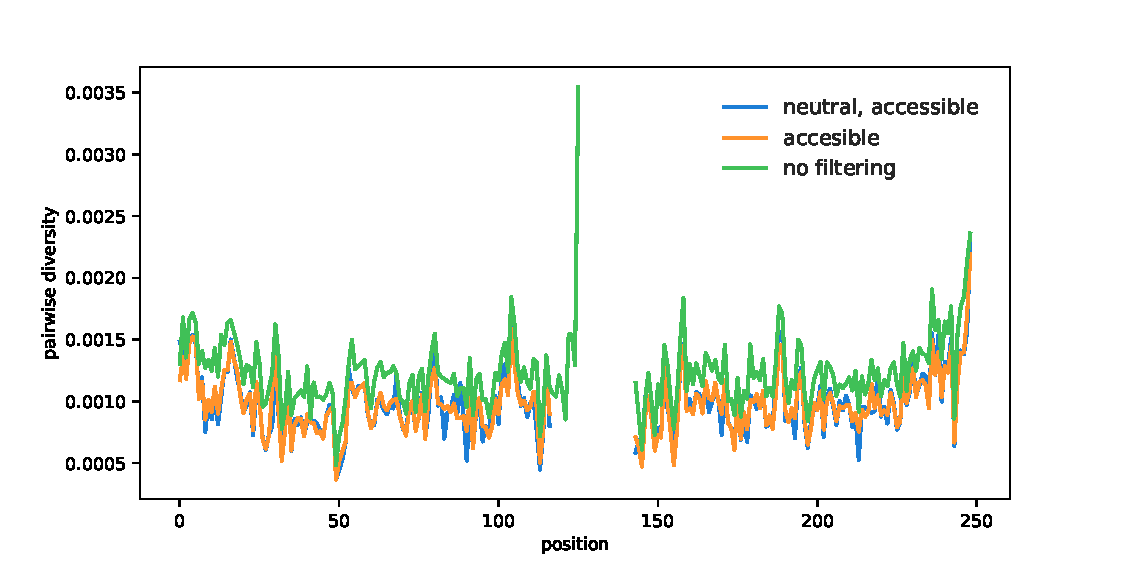
\includegraphics{figures/supplementary/chr1_diversity_filtering.pdf}

  \caption{Estimates of chromosome 1 YRI diversity in non-overlapping megabase
    windows, under different filtering criteria. The filtering criteria are,
    (1) ``neutral, accessible" which includes only putatively neutral sites, and
    ignores regions masked as inaccessible, (2) ``accessible" which is only ignores
  sites masked as inaccessible, and (3) ``no filtering" which uses all available
data. Note that filtering changes the absolute level of diversity, but has more
minor effects on regional patterns of diversity at the megabase scale.}

  \label{suppfig:chr1-diversity}
\end{figure}

\begin{table}
\centering
\begin{tabular}{lrrr}
  \hline
chrom &  accessible &  neutral &  both \\
  \hline
 chr1 &        42.4 &     64.4 &  22.9 \\
 chr2 &        46.8 &     58.7 &  23.7 \\
 chr3 &        44.1 &     62.9 &  24.8 \\
 chr4 &        44.0 &     59.3 &  21.5 \\
 chr5 &        44.1 &     58.0 &  21.4 \\
 chr6 &        45.0 &     58.0 &  22.1 \\
 chr7 &        44.4 &     65.8 &  26.4 \\
 chr8 &        43.8 &     61.2 &  23.1 \\
 chr9 &        39.2 &     64.5 &  20.3 \\
chr10 &        44.6 &     62.8 &  25.3 \\
chr11 &        42.7 &     63.5 &  23.4 \\
chr12 &        41.7 &     62.7 &  22.7 \\
chr13 &        39.7 &     62.0 &  18.3 \\
chr14 &        37.6 &     65.4 &  19.0 \\
chr15 &        37.0 &     69.4 &  20.3 \\
chr16 &        39.4 &     63.8 &  20.9 \\
chr17 &        40.4 &     64.0 &  22.3 \\
chr18 &        40.9 &     59.8 &  19.8 \\
chr19 &        30.9 &     69.8 &  18.0 \\
chr20 &        36.9 &     61.6 &  19.8 \\
chr21 &        31.6 &     68.6 &  18.2 \\
chr22 &        26.9 &     75.0 &  16.4 \\
\end{tabular}
\end{table}

\subsection{Data Summary Matrices}

Our underlying data for all likelihood and pairwise diversity estimates is the
allele count matrix $\mathbf{C}$ with dimensions $L \times 2$, where $L$ is the
chromosome length. This is transformed to a pairwise summary matrix with
identical dimensions, $\mathbf{Y}$. The first column of $\mathbf{Y}$ is the
number of pairwise comparisons between chromosomes that are identical, and the
second column is the number that are different. Both of these columns are
combinatoric summaries of the raw allele counts matrix needed for the binomial
likelihood and pairwise diversity estimates. Let $[c_1, c_2]$ be a row of
$\mathbf{C}$ for basepair $l$ (the $l$ index is omitted for clarity), and $n =
c_1 + c_2$. Then, the (1) total number of pairwise combinations of chromosomes
$n_T$, (2) the number of pairwise with identical alleles $n_S$, and (3) the
number of pairwise combinations with differing alleles $n_D$ are respectively,

\begin{align*}
  n_T &= \frac{n(n-1)}{2} \\
  n_S &= {c_1 \choose 2} + {c_2 \choose 2} \\
  n_D &= n_T - n_S
\end{align*}
%
which would be stored in row $\mathbf{Y}_l = [n_S, n_D]$. Note that the
per-site $\mathbf{Y}$ handles non-polymorphic sites and missing data.
Non-polymorphic sites have $n_S = {n \choose 2}$ and $n_D = 0$, and missing
data has $n_S = n_D = 0$.

\subsection{Pairwise Diversity Estimates}
\label{suppsec:diversity}

The pairwise diversity at site $l$ across the $n$ sampled chromosomes can be
calculated from row $l$ of the $\mathbf{Y}$ matrix as follows,

\begin{align}
  \pi_l = \frac{n_D}{n_T}
\end{align}

which is identical to the more common expression of this estimator, 

\begin{align}
  \pi_l = \frac{2}{n(n-1)} \sum_{i < j}^n k_{i,j}
\end{align}

where $k_{i,j}$ is 1 if the alleles at this site differ at site $l$, and 0
otherwise.

There are three ways to aggregate $\pi_l$ across all sites. The first is,

\begin{align}
  \label{eq:}
  \pi^{(1)} = \frac{1}{L} \sum_{i=1}^L \frac{n_{D,i}}{n_{T,i}}
\end{align}

which if the number of samples across loci is constant, simplifies to an
unweighted average across sites. Second, one can take a weighted average, with
weights determined by the total number of samples present at a site,

\begin{align}
  \label{eq:}
  \pi^{(2)} = \frac{1}{\sum_{i=1}^L n_i} \sum_{i=1}^L n_i \frac{n_{D,i}}{n_{T,i}}
\end{align}

Third, one can weight by the number of pairwise comparisons at a site,
$n_{T,i}$, rather than total number of samples, $n_i$, which leads to a ratio
of sums,

\begin{align}
  \label{eq:}
  \pi^{(3)} = \frac{\sum_{i=1}^L n_{D,i}}{\sum_{i=1}^L n_{T,i}}.
\end{align}

We predominantly use the estimator $\pi^{(3)}$, as it corresponds to how we
summarize the matrix $\mathbf{Y}$ across windows for our likelihood. All
methods have mean squared errors and biases very close to one another (TODO).

Note, however, that estimates of pairwise diversity often condition on the
accessible bases, and thus treat this as fixed. However, the number of
accessible bases varies across the chromosome; this can lead to a source of
apparent bias during block-bootstrap estimates of uncertainty.  In this case,
pairwise diversity is a ratio estimator, and is thus biased, since by Jensen's
inequality $\E(\nicefrac{y}{x}) \ge \nicefrac{\E(y)}{\E(x)}$ for random
variables $x$ and $y$. 

\subsection{Window-based Summaries and filtering}

\begin{figure}[!htb]
  \centering
  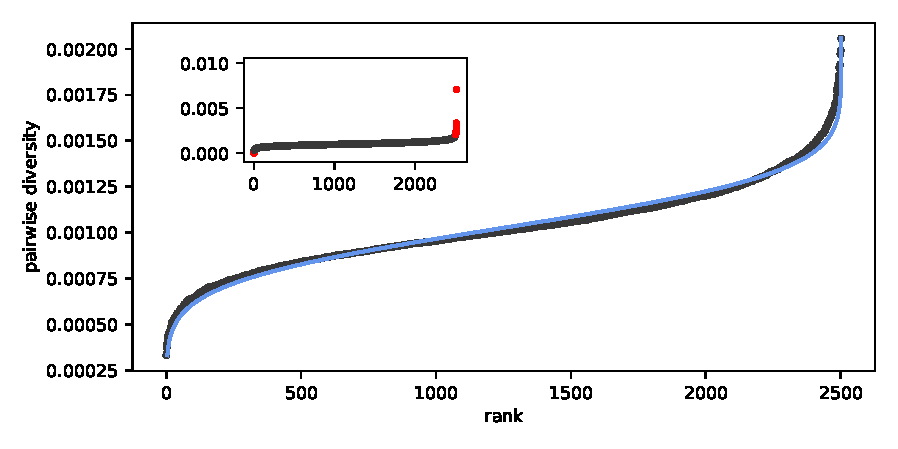
\includegraphics{figures/supplementary/diversity_trimming_dist.pdf}

  \caption{The distribution of diversity across the genome at the megabase
  scale, with outliers trimmed. The blue line is the normal CDF, fit with MLE
parameters XXX. The inset figure is the untrimmed data, with trimmed points
shown in red.}

  \label{suppfig:trimming}
\end{figure}



The likelihood method is fit to non-overlapping binned summaries of the allele
counts matrix. 


Based on exploratory data analyses, some bins were outliers and
excluded (XXX).

\begin{enumerate}
  \item \textbf{Fraction of inaccessible sites per window}.  \path{mask_inaccessible_bins_frac}
  % \item \textbf{Edge truncation}

  \item \textbf{Outliers}: Based on exploratory analysis, there were some
    regions with very high diversity. The 0.05\% right tail was excluded.

\end{enumerate}


% supp data
% - npy files
% - edge trunation

\section*{Likelihood}

Our model is essentially a generalized nonlinear model with a binomial link
function. This is the form used by \textcite{Elyashiv2016-vt} and
\textcite{Murphy2022-sj}. These models fit the observed number of pairwise
nucleotide differences in genomic windows to the expected pairwise diversity
under some evolutionary model. We only consider BGS models here, so the mean
function for position $x$ is the product of the proportion by which BGS reduces
diversity at position $x$, $B(x)$, and genome-wide neutral diversity $\pi_0$,

\begin{align}
  \pi(x) = B(x, \Phi) \pi_0
\end{align}

$\Phi$ is the set of BGS parameters (i.e. the DFE for each feature type and
mutation rate), and $\pi_0 = 4 N_e \mu$ is determined by the genome-wide
drift-effective population size $N_e$, set by only reproductive and demographic
processes. Regional mutation rate heterogeneity can be accounted for with a
regional mutation rate scaling function $m(x)$, $\pi(x) = B(x, \Phi) m(x)
\pi_0$, but we do not explore mutation-rate heterogeneity, as it is unclear how
to differentiate variance in mutation rate from the substitution rate
heterogeneity we find across the genome.

The likelihood of the set of parameters $\Psi = \{\pi_0, \Phi\}$ can be written
in the form of, 

\begin{align}
  \log\mathcal{L}(\Psi) = \sum_{v \in \mathcal{V}} \sum_{i \ne j \in \mathcal{S}} \log(P(O_{i,j}(v) | \Psi))
\end{align}

(c.f. \cite{McVicker2009-ax,Elyashiv2016-vt,Murphy2022-sj}) where $\mathcal{V}$
is the set of putatively neutral sites, $\mathcal{S}$ is the set of samples,
and $\Psi$ are the BGS parameters. The indicator variable $O_{i,j}(v)$ is 1 if
samples $i$ and $j$ are different at putatively neutral site $v$, and zero
otherwise. While the theoretic $\pi(v)$ gives the average number of pairwise
differences, for small values, this is approximately the heterozygosity
probability, so we can write

\begin{align}
  P(O_{i,j}(v) | \Psi) = 
    \begin{cases}
      \pi(v), & O_{i,j}(v, \Psi) = 1 \\
      1-\pi(v), & O_{i,j}(v, \Psi) = 0 \\
    \end{cases}.
\end{align}

(c.f. \cite{Elyashiv2016-vt}). 

As in Section \ref{suppsec:diversity}, the number of pairwise differences and
the total number of pairwise comparison at a site are sufficient statistics for
the likelihood. Then, the binomial log-likelihood for the data at site $v$ is,

\begin{align}
  \ell_v(\Psi) &= \log(\pi(v, \Psi)) n_{\text{D},v} + \log(1-\pi(v, \Psi)) n_{\text{S},{v}}
\end{align}

\subsection{The scale of processes}

We can observe $\widehat{\pi}(x)$ at a per-basepair resolution. However, for a
variety of reasons, we do not want to fit the composite likelihood model to the
per-basepair scale of data. First, this would be computationally infeasible.
Second, the mean function $\pi(x)$ varies on a natural scale that is itself a
free parameter of the model. Our model can be written as, 

\begin{align}
  \ell(\Psi, h) &= \sum_{b} \sum_{v \in \mathcal{V}_b} \ell_v(\Psi) \\
             &= \sum_{b} \left[\log(\bar{\pi}(b, \Psi)) \sum_{v \in \mathcal{V}_b} n_{\text{D},v} + \log(1-\bar{\pi}(b, \Psi)) \sum_{v \in \mathcal{V}_b} n_{\text{S},{v}}\right] \\
             &= \sum_{b} \left[\log(\bar{\pi}(b, \Psi)) Y_{\text{D},b} + \log(1-\bar{\pi}(b, \Psi)) Y_{\text{S},{b}}\right] \\
\end{align}

where $h$ is the bandwidth or window size, $b$ the bin index for windows of
width $h$, $\mathcal{V}_b$ is the set of putatively neutral sites in bin $b$,
$\bar{\pi}(b | \Psi)$ are the average diversity in bin $b$, and
$Y_{\text{S},b}$ and $Y_{\text{S},b}$ are the sums across putatively neutral
sites within a bin. Note that by binning, we sum the pairwise summaries of the
data $\mathbf{Y}$ across sites, so the likelihood across bins is naturally
weighted by the quantity of observed data. We estimate $h$ by fitting the model
for a variety of window sizes $h$ and select the best using out-sample cross
validation, as is standard in non-parametric regression (XXX, Wasserman, p.
70).

This model corresponds to a binomial likelihood for the observed data
summarized at genomic scale $h$. Thus an alternative way to express this model
is as, 

\begin{align}
  Y_{\text{D},b} \sim \text{Binom}(\bar{\pi}(b, \Psi), Y_{\text{D},b} + Y_{\text{S},b}).
\end{align}

Here, $\bar{\pi}(b, \Psi)$ is assumed to be the \emph{probability} of sampling
two different alleles, rather than the average \emph{number} of pairwise
differences; these are approximately equal when $\pi$ is small. This
corresponds to an identity link function; one could alternatively use a
two-alleles finite sites model link function of the form, $\pi/(1 + 2 \pi)$. We
experimented with this and found there was little difference between these link
functions, so we opted for the simpler identity link function.


\section{Background Selection Models}

The BGS models considered here both assume multiplicative fitness effects
across sites. Thus, the total reduction due to segments across the genome is
the product of the individual reductions, 

\begin{align}
  \label{suppeqn:b}
  B(x, \Psi) = \prod_g^S \int_0^1 b(\mu(s, k(g)), s, L_g, r_g, d(x, g)) ds
\end{align}

where, $b(\mu(s, k(g)), s, L_g, r_g, d(x,g))$ is the reduction due to segment
$g$, and there are $S$ total segments. Here, $\mu(s, k(g))$ is the per-basepair
per-genome rate that mutations with selection coefficient $s$ enter segments
with feature class $k(g)$, $L_g$ and $r_g$ are the length in basepairs and
recombination rate per basepair of segment $g$, and the recombination distance
between focal site $x$ and segment $g$ is $d(x, g)$. The functional form of $b$
varies depending on whether the classic BGS model is used, or our form of
Santiago and Caballero's (\citeyear{Santiago2016-mu}) equations (see Section
XXX).

Under both background selection models used in our likelihood, the diversity in
window $b$ is $\bar{\pi}(b, \Psi) = \bar{B}(b, \Psi) \pi_0$. Here, $\bar{B}(b |
\Psi)$ is the predicted reduction in diversity due to BGS in window $b$, given
background selection parameters $\Psi$. In practice, we pre-calculate $B(x |
\Psi)$ at fixed sites $x$ across the genome, and take the average of the fixed
sites $B$ values within widow $b$ for the average $\bar{B}(b | \Psi)$. 

\subsection{Reductions Under the Classic BGS Model}

The classic BGS model, which assumes deleterious mutations cannot fix,
expresses the reduction for a focal site in the middle of a segment
\parencite{Hudson1995-xc,Hudson1994-oh,Nordborg1996-nq}; here we consider a
focal site directly to an arbitrary side of a segment under a deleterious
mutations, and extend the model to handle a focal segment arbitrarily far from
the segment. To simplify notation, we will only consider a single feature class
in this and the next section. Using our notation from equation
\eqref{suppeqn:b}, the classic mutation-selection-balance BGS model is,

\begin{align}
  b(\mu, s, L, r, 0) &= \exp \left( - \int_0^L \frac{2\mu(l)}{s (1 + (1-s) r(l)/s)^2} dl \right) 
\end{align}

(c.f. \cite{Hudson1995-xc} equation 5), where $\mu(l)$ is the \emph{haploid}
per-basepair mutation rate at $l$ and $r(l)$ is the recombination fraction
between the focal site (at position 0) and basepair $l$. Assuming constant
per-basepair recombination and mutation rates, $r(l) = r_\text{BP}l$ and
$\mu(l) = \mu$, and

\begin{align}
  b(\mu, s, L, r_\text{BP}, 0) &= \exp \left( - \frac{2\mu L}{s + (1-s) r_\text{BP} L} \right)
\end{align}

(c.f. \cite{Hudson1995-xc} equation 8, where the factor of two difference is
due to the position of the focal site). Often per-region rates are defined $U =
2 \mu L$ and $M = r_\text{BP} L$ are the segment-wide mutation diploid mutation
rates (mutations per diploid segment per generation) and recombination length
(Morgans). 

For computational efficiency, we adjust this model by setting $r(l) = d +
r_\text{BP} l$, where $d$ is the recombination fraction between the focal site
$x$ and the start of segment $g$. This allows us to pre-compute the local
effects of the segment, and substitute in $b$ as the focal site changes. This
integral substitution has a closed form,

\begin{align}
  b(\mu, s, L, r_\text{BP}, d) &= \exp \left( \frac{-2\mu L}{(d(1-s) + s)(s + (d + r_\text{BP}L)(1-s))} \right)
\end{align}

and terms can be collected in powers of $d$ and pre-computed for all segments
for the grid of $\mu$ and $s$. Our implementation pre-computes these segment
components, and computes the final $b$ value for an $x$ and $g$ by calculating
the distance $d(x,g) = |M(x) - M(g)|$, where $M(x)$ is the cumulative
recombination map length at position $x$ in Morgans. Since $r(l)$ could vary by
position, segments with differing recombination rates are split into segments
of the same annotation class by their recombination rate. This has no effect on
the calculation due to the multiplicative fitness, but ensures more accurate
estimates of the reduction factor $B$.

% Each B map is determined by the annotation track of putatively conserved
% segments, which includes (1) the segment positions and lengths, (2) the type of
% feature of each segment (e.g.  exons, UTRs, phastcons conserved elements,
% etc.), as well as (3) the recombination map, and (3) the deleterious selection
% coefficient $s(i)$ and mutation rate at which these deleterious enter the
% population for feature type $i$.

\subsection{Reduction Under the Modified Santiago and Caballero Model}

When weak deleterious mutations can fix, causing substitutions, the classic
background selection models break down. We find that the generalized background
selection model of \textcite{Santiago2016-mu} works well (see Section XXX for
our derivation). Unlike the classic BGS models which only produce B maps, that
only estimate the reduction in effective population size, The generalized BGS
model of \textcite{Santiago2016-mu} also predicts the deleterious substitution
rate per generation per segment (the ``ratchet" rate), which we call the R map.
We describe how these are calculated substitution rates per segment, for each
mutation rate and selection coefficient combination in the grids. We describe
how these are calculated here.

First, the reduction factor experienced by a focal site within the segment $g$
(and thus is similar to what selected alleles in $g$ experience) under
generalized background selection is calculated as

\begin{align}
  \widetilde{b}'(\mu, s, L, r_\text{BP}) = \frac{\widetilde{N}_{e,\infty}}{N}
\end{align}

where $\widetilde{N}_{e,\infty}$ is the asymptotic effective population size,
which is the solution to the following system of two equations (see XXX for
derivation),

\begin{align}
  {N}_{e,\infty} &= N \exp \left( -\frac{V}{2} Q_\infty^2 \right) \\
  {R} &= \frac{4 U s N_{e,\infty}}{\exp(4 N_{e,\infty} s)-1}\\
\end{align}

where 

\begin{align}
  V &= U s - 2 {R} s \\
  Q_\infty^2 &= \frac{2}{(1-Z)(2-(2-M)Z)} \\
  Z &= 1 - \frac{Us}{U-{R}}
\end{align}

and $U = 2\mu L$ and $M = r_\text{BP} L$ as above. In this section, we assume
$\mu$ is the mutation rate to variants with heterozygous selection coefficient
$s$ to simplify notation; later, $\mu$ refers to the genome-wide average
mutation rate and the mutation rate is scaled by the DFE. Solving this system
of two equations for each segment also gives the total substitution or
``ratchet" rate per generation per segment ($\widetilde{R}$). The per-basepair
substitution rate of a segment with mutation rate $\mu$ and selection
coefficient $s$ is $\lambda_d(\mu, s) = \nicefrac{\widetilde{R}}{L}$

Under Santiago and Caballero's model, the correct effective population size to
gauge reduction in heterozygosity or coalescent times is given by equation XXX.
This is because selective processes can lead to non-constant pairwise
coalescent rates, which impact pairwise coalescent rates and thus the reduction
factor. We experimented with the corrections described in Section XXX, and
found (1) they had little effect on the accuracy of the B maps, and (2) they
were incredibly costly to calculate, even with the approximations described in
equations XXX. Overall, we solve for the asymptotic $\widetilde{N}_{e,\infty}$
for each segment, and use that to calculate $b'$.

Note that the asymptotic model above determines the reduction in effective
population size experienced by a focal site in the middle of a $L$-basepair
segment, but B maps require the reduction $b'$ experienced by a focal site $x$
at an arbitrary recombination distance apart. For each segment, we pre-compute
the solution to the system of two equations, giving us $V$ and $Q_\infty^2$,
and then use these values in the equation,

\begin{align}
  b'(\mu, s, L, r, d) = \exp\left( -\frac{V}{2} \left(\frac{1}{(1-(1-d)Z}\right)^2 \right) 
\end{align}

where $Z = 1 - Us / (U-\widetilde{R})$ and $V = Us - 2\widetilde{R}s$.


\subsection{Discretization of Parameters and Annotation Feature Classes}

\begin{align}
  \label{suppeqn:b}
  B(x, \Psi) = \prod_g \sum_{i} b(\mu_{i, \;k(g)}, s_i, L_g, r_g, d(x, g))
\end{align}

In practice, to fit such a model, we must discretize both $\mu(s, k(g))$ and
$s$. Our models use a fixed $m_s$-element grid of selection coefficients, and
mutation rates are on a fixed $m_\mu$-element grid, which is later interpolated
over during the maximum likelihood optimization. The number of annotation
features $K$ is variable and set by the annotation data specified. There are
two ways to parameterize the mutation rates and DFE for all annotation classes
in background selection models. First, for the \emph{free-mutation}
parameterization, each annotation feature class has a free mutation rate
parameter for each of these selection coefficients (as in equation
\eqref{suppeqn:b}).

In the free-mutation parameterization, there are $1 + K \times m_s$ for $\pi_0$
and the free mutation rate parameters, where $K$ is the number of annotation
features. The MLE optimization for this approach is unconstrained, though
$\pi_0$ is bounded to be within $10^{-5} \le \pi_0 \le 10^{-1}$ and mutation
rates are bounded within $10^{-11} \le \mu \le 10^{-7}$. The BGS model requires
a mutation rate for each selection coefficient in the grid, for each annotation
class (here, as an example, CDS, UTRs, and phastcons), which are stored in the
$m_s \times K$ matrix $\mathbf{M}_\text{F}$,

\begin{align}
  \mathbf{M}_\text{F} = \begin{bmatrix}
    \mu_{10^{-6},\text{CDS}} & \mu_{10^{-6},\text{UTR}} & \mu_{10^{-6},\text{PC}} \\
    \mu_{10^{-5},\text{CDS}} & \mu_{10^{-5},\text{UTR}} & \mu_{10^{-5},\text{PC}} \\
    \vdots & \vdots & \vdots \\
    \mu_{10^{-1},\text{CDS}} & \mu_{10^{-1},\text{UTR}} & \mu_{10^{-1},\text{PC}} \\
  \end{bmatrix}
\end{align}

That is, the distribution of fitness effect (DFE) is implied by
the total mutation rate across selection coefficients for an annotation class.
We can normalize by the total mutation rate estimate to get the estimated DFE,
giving us the DFE weight for annotation class $k$ and selection coefficient
with index $i$,

\begin{align}
  \widehat{w}_{i,k} = \frac{\widehat{\mu}_{i,k}}{\sum_i \widehat{\mu}_{i,k}}.
\end{align}

The second parametrization is the \emph{simplex} parametrization, which has a
single mutation rate across all features, so it is a DFE weight matrix times
the mutation rate $\mu$, 

\begin{align}
  \mathbf{M}_\text{S} = \mu \begin{bmatrix}
    w_{10^{-6},\text{CDS}} & w_{10^{-6},\text{UTR}} & w_{10^{-6},\text{PC}} \\
    w_{10^{-5},\text{CDS}} & w_{10^{-5},\text{UTR}} & w_{10^{-5},\text{PC}} \\
    \vdots & \vdots & \vdots \\
    w_{10^{-1},\text{CDS}} & w_{10^{-1},\text{UTR}} & w_{10^{-1},\text{PC}} \\
  \end{bmatrix}
\end{align}

which has $2 + K \times (m_s-1)$ free parameters, since each column must sum to
one. This imposes the constraint that $\sum_i w_{i,k} = 1$, requiring
constrained MLE optimization. 

\section{Ratchet Rate Prediction}

After rescaling each segment $N_e$ by the local predicted reduction
$\hat{B}(x)$, the ratchet rates and $B'$ values are re-calculated. 

The rescaled $B'$ calculation outputs a $m_\mu \times m_s \times S$
multidimensional array $\mathbf{R}$ of ratchet rates per segment. These are
rescaled by the segment lengths $\mathbf{l}$, giving the per-basepair mutation
rate array. The per-basepair ratchet rate given maximum likelihood estimates of
$\hat{\mu}$ and $\widehat{\mathbf{W}}$ is used to predicted the ratchet rate
for each segment $g$. The DFE estimate for feature $k$ is a column vector of
$\widehat{\mathbf{W}}$, i.e. $\widehat{\mathbf{w}}_k$

\begin{align}
  \lambda_D(g) = 
\end{align}

The predicted ratchet rate for segment $g$ $\lambda_d(g)$ is based on these
values.

\printbibliography

\end{document}
